%!TEX root = ../main.tex

\chapter{The background after the LAr veto cut}\label{chap:bkg:lar:ph2}

All what has been shown until now concerns data before the LAr and PSD cut. In this
chapter a model of the background after the LAr veto cut will be presented, based on a
Monte Carlo simulation of the LAr scintillation light propagation. Being able to describe
the background after this major event selection is indeed of great interest to study the
distribution of two-neutrino double-beta decay events, which are almost never vetoed by
the LAr veto system. As extensively shown in \cref{chap:theory}, the presence of several
new physics phenomena can be constrained by looking at the shape of the \nnbb\ events
distribution. Understanding the action of the LAr veto cut on background events from the
point of view of the background model requires, however, a full Monte Carlo simulation of
the LAr scintillation mechanism as well as the implementation of all the relevant material
and surface optical properties that contribute to light propagation in the \gerda\ experimental
setup. Implementing such a simulation, as it will be shown, requires an accurate knowledge
of many optical parameters, which is not always the case, unfortunately, with the \gerda\
setup. Nevertheless, it is possible to use special calibration data with low-activity
sources and the LAr veto instrumentation turned on to constrain the LAr veto Monte Carlo
model. An independent analysis of this special data set is used to tune the unknown
optical parameters in the Monte Carlo such to reproduce the observed vetoing performance.
The obtained parameters are then used to produce a map of the LAr scintillation light
detection probability, which is applied to the background model simulations in order to
obtain the LAr veto flag. Based on these new background model pdfs, a statistical analysis
to test possible deviations of the \nnbb\ distribution from its Standard Model description
will be finally presented.
\newpar
The chapter is structured as follows: \fillme{fillme}

\section{Optical physics in \mage}%
\label{sec:bkg:lar:ph2:mage}

Optical materials and surfaces are implemented in \mage\ through the relevant \geant\
libraries. Once properties like reflectivity, wavelength-shifting capabilities,
attenuation lengths, scintillation yields etc.~are defined, the \geant\ core routines take
care of simulating light propagation accordingly. When defining optical parameters in the
Monte Carlo, one must keep in mind what are the typical photon wavelengths that come to
play in the \gerda\ setup. The most important wavelength is 128~nm, in the so-called
vacuum-ultra-violet (VUV) regime, which defines the energy of the photon emitted by the
LAr scintillation process. The second interesting regime is in the 400--600~nm range,
typical of photons which are wavelength-shifted (WLS) in the fiber curtain or by
Tetraphenil-Butadiene (TPB) coatings to match the absorption range of the light detectors
(PMTs, SiPMs). As it will be clear in the next sections, many optical parameters are
poorly known in the VUV regime or depend on the details of the experimental setup (LAr
purity, WLS coating thickness etc.), and a dedicated measurement should be therefore
performed.  In the following sections a reference list of the optical properties
implemented in \mage\ is provided, with references to the literature.

\blocktitle{liquid \\ argon}
Key properties of the liquid argon from the point of view of the vetoing performance in
\gerda\ are the scintillation mechanism, the refractive index and the attenuation length.
The first two are relatively well known, while the latter strongly depends on the LAr
purity, which has not been measured for \gerda. We recall here that the deployed LAr has
not been subject to any purification process, and is therefore expected to meet the purity
specifications of natural argon.

\begin{description}

  \item[Refractive index] Its implementation is dependent on the photon energy (shown in
    \cref{fig:bkg:lar:ph2:mage:lar-props}). Formulas are taken from~\cite{Bideau-Mehu1981}
    and give about 1.41 at 128~nm. A more recent measurement, similarly based on an
    extrapolation of measured data to lower wavelengths, suggests a lower value of about
    1.37~\cite{Babicz2018}.

  \item[Rayleigh scattering length]. Depends on the refractive index and therefore the
    photon energy (shown in \cref{fig:bkg:lar:ph2:mage:lar-props}). Formulas are taken
    from~\cite{Seidel2002}. The already implemented refractive index values are used. The
    obtained scattering length value at 128~nm is about 60~cm. The value suggested
    in~\cite{Babicz2018} is 91~cm, 50\% higher.

  \item[Scintillation spectrum] Taken from~\cite{Heindl2010}, which reports an
    experimental measurement (fig.~1 and 2). Only the (gaussian) peak is implemented in
    \mage, as the non-gaussian contributions are of several orders of magnitude lower and
    are therefore negligible. A normal distribution $(\mu=128\;\text{nm},
    \sigma=2.929\;\text{nm})$ is implemented (\cref{fig:bkg:lar:ph2:mage:lar-props}).

  \item[Scintillation yield] Different scintillation processes are defined in the \mage\
    physics list for different ionizing particles, that in general have different
    scintillation yields in LAr. A default, reference value of $51\;\upgamma/\text{keV}$
    is set for all particles~\cite{Doke2002}. This value does certainly not represent the
    reality of \gerda, as the yield strongly depends on the electric field configuration
    and the quencher impurities. Unfortunately a a reliable direct measure of the
    scintillation yield of the \gerda\ LAr is not available.  Indirect measurements were
    performed within the \LArGe\ setup~\cite{Lehnert2015} and with a dedicated setup
    deployed inside the \gerda\ cryostat~\cite{Barros2020}, but they both yield
    incompatible results. As shown in~\cite{Doke2002}, some particles, interestingly \a\
    particles and nuclei, can have lower yields. Therefore, the photon yield is reduced
    for \a\ particles and nuclei by a factor of 0.875 and 0.375 respectively in the
    physics list. These numbers are extracted from~\cite{Doke2002}. In this way \b\ and
    \g\ particles will be affected by the nominal (maximum) photon yield, while \a\
    particles and nuclei will produce less light by a factor 0.875 and 0.375 (0.7/0.8 and
    0.3/0.8 according to~\cite{Doke2002}), respectively.

  \item[Singlet and triplet lifetime] \sloppy The implemented triplet lifetime is the one
    measured during \gerdatwo, before the \phasetwop\ upgrade
    (\cref{fig:lar:triplet-lifetime}), the singlet lifetime \fillme{fillme}. The relative
    occurrence of the two de-excitation processes is also specified in terms of
    scintillation yield. The \geant\ \m{YIELDRATIO} property, which is defined as the
    relative strength of the fast component as a fraction of total scintillation yield, is
    set to 0.23 for all particles (\b\ and \g\ particles), 0.75 for nuclei and 1.0 for \a\
    particles (the latter is a rough guess).

  \item[Attenuation length] As the absorption length is strongly dependent on the LAr
    purity, no literature values can be used. It is known to depend on the wavelength of
    the photon in general, but this dependence is poorly known in the VUV regime. What is
    most important in \mage\ is its value at 128~nm, i.e.~the wavelength of the LAr
    scintillation light. The following, heuristic implementation is adopted: an
    exponential function is used to make sure that the LAr is opaque to VUV photons
    ($\lambda \leq 128$~nm) but transparent to wavelength-shifted photons ($\lambda
    \gtrsim 400$~nm), see fig.~\ref{fig:bkg:lar:ph2:mage:lar-props}. A measurement of the
    attenuation length in the \gerda\ LAr was performed~\cite{Barros2020}, yielding
    $\sim15$~cm as a result, but \fillme{fillme}

  \item[Fano factor] A Fano factor of 0.11 is set, taken from~\cite{Doke1976}.

\end{description}

\begin{figure}
  \centering
  \includegraphics{plots/mage/lar-props.pdf}
  \caption{%
    LAr optical properties as implemented in \mage. Top left: the refractive index, top
    right: the Rayleigh absorption length, bottom left: the scintillation spectrum, bottom
    right: the absorption length. Taken from~\cite{Bideau-Mehu1981, Seidel2002,
    Heindl2010}.
  }\label{fig:bkg:lar:ph2:mage:lar-props}
\end{figure}

\blocktitle{reflectivity}
Reflectivity is another key property in optical simulations, as it can be different for
VUV scintillation photons and wavelength-shifted photons. Unfortunately, the available
literature about material reflectivity in the VUV regime is often very scarce. Surfaces
in the \gerda\ setup for which knowing the reflectivity is crucial are certainly
germanium, silicon holder plates and the VM2000 and Tetratex\reg{} reflectors that cover
the internal copper surface of the LAr veto instrumentation.

\begin{description}
  \item[Ge, Si, Cu and Teflon] Measurements performed for \gerda\ are available
    in~\cite{Wegmann2017}.  A reflectometer at room temperature and in air was used to
    measure the reflectivity in the wavelength range $[280, 700]$~nm, therefore values in
    the VUV region must be taken from other sources. For germanium it seems to strongly
    depend upon the radiation incident angle~\cite{Marton1967}, but it's not possible to
    implement angle-dependent reflectivities in \geant\ yet. A rough, average value of
    0.65 is therefore set for wavelengths smaller than 280~nm. The source of the
    reflectivity values of the other materials below 280~nm is not known to me
    \fillme{fillme}. The reflectivity values for all materials mentioned above are plot in
    \cref{fig:bkg:lar:ph2:mage:metals-refl}.

    \begin{figure}
      \centering
      \includegraphics{plots/mage/metals-refl.pdf}
      \caption{%
        Reflectivity of germanium, copper, silicon and Teflon as implemented in \mage.
      }\label{fig:bkg:lar:ph2:mage:metals-refl}
    \end{figure}

  \item[Polymeric reflectors] Tetratex\reg{} values are taken from~\cite{Janecek2012}. The
    author reports measurements of the reflectivity of 2 and 4 superimposed layers of
    160~\mum\ thick Tetratex\reg{}. As the thickness of the foils used in \gerda\ is
    254~\mum, the results for the two superimposed foils (320~\mum) are implemented in
    \mage. In reality, the reflectivity of the \gerda\ foils should be (negligibly)
    smaller. The TPB layer has some effect on the reflectivity, but there's no measurement
    available in literature.  VM2000 values are taken from~\cite{Francini2013}.  The
    authors report measurements of TPB-coated VM2000, as in the \gerda\ setup, which then
    take into account the effect of the TPB emission spectrum. The measurement seems to be
    independent on the TPB layer thickness. The values are plot in
    \cref{fig:bkg:lar:ph2:mage:misc}, left.

    \begin{figure}
      \centering
      \includegraphics{plots/mage/misc.pdf}
      \caption{%
        Reflectivity of VM2000 and Tetratex\reg{} reflectors (right) and absorption length
        of the nylon mini-shrouds (left), as implemented in \mage.
      }\label{fig:bkg:lar:ph2:mage:misc}
    \end{figure}

\end{description}

\blocktitle{wavelength \\ shifters}
Various surfaces in the \gerda\ setup are coated with a wavelength-shifting material in
order to enhance the light collection efficiency and therefore the LAr veto cut
efficiency. Tetraphenyl-Butadiene (TPB) is either evaporated on the surface pure or
embedded in a polystyrene matrix. The concerned surfaces are the nylon mini-shrouds, the
light-guiding fibers, the VM2000 and Tetratex\reg{} reflectors on the copper components of
the LAr veto instrumentation (or simply copper shrouds in the following) and the PMTs
glass window. The physical properties that define the wavelength-shifting process are the
quantum efficiencies (average number of WLS photons emitted), the emission spectrum of the
emitted WLS photons and their absorption length in the material. Since these properties
depend on the substrate and other characteristics like the thickness or the deposition
technique, multiple definitions of TPB are present in \mage. The quantum efficiency
depends on the layer thickness, so it should be measured for the specific sample. Since
these measurements are not available, an arbitrary but realistic value of 1.2 is set. The
WLS absorption length is another property for which no good data seems to be available in
the literature. The implemented values are taken from~\cite{Benson2017}
(\cref{fig:bkg:lar:ph2:mage:tpb-props}, left). Other TPB properties which are common to
all instances are the WLS emission time constant, which is set to an arbitrarily small
value of 0.01~ns and the reflectivity which should be small but not zero (set to 0.2).
The WLS emission spectrum changes upon the specific layer

\begin{description}

  \item[TPB on nylon mini-shrouds] This WLS coating consists of TPB embedded in a
    polystyrene matrix (3:7 ratio TPB:polystyrene) and diluted in toluene (1:10).  The
    solution is then brushed on the nylon. The emission spectrum has been
    measured~\cite{Walter2015} (see \cref{fig:bkg:lar:ph2:mage:tpb-props}, right) and is
    similar to the one in reported~\cite{Francini2013} (fig.~14) for TPB in polystyrene
    matrix on glass.

  \item[TPB on VM2000] The copper shroud internal reflective surface is coated with
    evaporated TPB. The emission spectrum is taken from~\cite{Francini2013}
    (\cref{fig:bkg:lar:ph2:mage:tpb-props}, right).  The authors report the measurement of
    a $\sim$160~\mum\ thick TPB layer on VM2000 at an excitation wavelength of 128~nm and
    at 87~K, the same \gerda\ experimental conditions. The major differences brought in by
    the LAr temperature are the vibronic structures that modify the shape of the spectrum.

  \item[TPB on fibers] No measurement is available here so the same emission spectrum
    defined for TPB on VM2000 is used. The TPB is evaporated.

  \item[TPB on Tetratex\reg{}] The Tetratex\reg{} is dip-coated (0.9~mg/cm$^2$, 8~\mum\
    thickness) with TPB. The emission spectrum has been measured for
    \gerda~\cite{Baudis2015a} and is reported in \cref{fig:bkg:lar:ph2:mage:tpb-props},
    right. The measured sample has a TPB surface density of 0.17~mg/cm$^2$. In principle
    the thickness affects the shape of the emission spectrum, as the efficiency of the
    reabsorption effect increases with the thickness of the layer. However, no relative
    measurements could be found at the time.

    \begin{figure}
      \centering
      \includegraphics{plots/mage/tpb-props.pdf}
      \caption{%
        Optical properties of Tetraphenyl-Butadiene (TPB) implemented in \mage. On the
        left: the attenuation length of the wavelength-shifted light. On the right:
        emission spectrum.
      }\label{fig:bkg:lar:ph2:mage:tpb-props}
    \end{figure}

\end{description}

\blocktitle{fiber shroud \\ mini-shrouds}
An essential part of the LAr veto system is the wavelength-shifting light-guiding fiber
curtain. The fibers themselves are a Saint Gobain product (BCF-91A polystyrene
fibers~\cite{FibersData}), and consist of a core and two cladding layers with different
refraction indices, to increase the light trapping efficiency, which is of about 3\%.
Photons interacting in the fiber are shifted to the green band of the optical spectrum,
guided to the endpoints and collected by the SiPMs at the top. The fibers are coated with
TPB, that shifts the VUV light to match the fiber absorption range.
\newpar
The nylon mini-shrouds have the triple role of keeping \kvz\ ions out, being transparent
to optical photons and eventually shift VUV photons to higher wavelengths. This capability
is achieved by coating them with TPB.

\begin{description}

  \item[BCF-91A polystyrene] Material of the fiber core. The data sheet from Saint
    Gobain~\cite{FibersData} reports the absorption spectrum, knowing that the fibers are
    1~mm thick one can extract the absorption length. Starting from the trivial relation:
    \[
      1 - P(E) = e^{-x/l(E)}
    \]
    where $P(E)$ is the probability (thus proportional to the absorption
    spectrum) for a photon travelling a distance $x$ to be absorbed in the
    material. Given the attenuation length $l(E)$, one can extract $l(E)$ from
    $P(E)$. By integrating over the thickness of the material $L$ one obtains:
    \[
      L \cdot (1 - P(E)) = l(E) \cdot (1 - e^{-L/l(E)})
    \]
    The problem now is that $l(E)$ cannot be extracted analytically (the expression is
    inhomogeneous). It can however be solved numerically.  Since the units are arbitrary
    because the original absorption spectrum has arbitrary units, the spectrum has been
    then rescaled to match a measurement performed at 400~nm, which yielded
    0.7~mm~\cite{Raphael Kneissl's bachelor thesis}. The result is shown in
    \cref{fig:bkg:lar:ph2:mage:fibers-props}, left. The emission spectrum is taken again
    from~\cite{FibersData} and shown in \cref{fig:bkg:lar:ph2:mage:fibers-props}, right.
    The absorption length is set to 3.5~m \fillme{fillme}. The WLS time constant, the
    refractive index have also been taken from~\cite{FibersData}. The quantum efficiency
    is set to 1. The two cladding layers are made of PMMA. As only the refractive index is
    important, it is set to 1.49 for the inner cladding layer and to 1.42 for the outer
    layer~\cite{FibersData}.

  \item[Nylon mini-shrouds] The refraction index is set to 1.54, constant over
    incident photon wavelength. The attenuation length values are taken
    from~\cite{Agostini2017a}, since \gerda\ is using the same material used for the
    \textsc{Borexino} balloon (\cref{fig:bkg:lar:ph2:mage:misc}, right).

    \begin{figure}
      \centering
      \includegraphics{plots/mage/fibers-props.pdf}
      \caption{%
        Absorption length and emission spectrum of the wavelength-shifted light in the
        light-guiding fibers, as implemented in \mage.
      }\label{fig:bkg:lar:ph2:mage:fibers-props}
    \end{figure}

\end{description}

\section{Simulating the LAr veto}%
\label{sec:bkg:lar:ph2:heatmap}

Simulating optical physics is notoriously a computationally intensive task, as the number
of photons to track is very high. Enabling optical processes in background model
simulations, which already take tens of thousands of CPU hours to complete, is not
feasible. To address the issue, an alternative approach to compute the LAr veto flag for
already existing simulations has been developed, based on the construction of a detection
probability map of scintillation photons in LAr. This object, which is going to be
described in this section, will be also be referred to simply as `heat map' or
`probability map' in the following.
\newpar
The first step to produce the probability map is to run a full photon tracking simulation
of 128~nm scintillation photons in the whole LAr volume defined in \mage. An isotropic
source of VUV photons homogeneously distributed in a pre-selected LAr volume is simulated.
\mage\ allows to restrict the sampling to the volume occupied by LAr only or its
intersection with a geometric solid (e.g.~a cylinder). The photon initial energy is
sampled from a Gaussian distribution with mean 128~nm and variance 2.929~nm. After being
propagated in the implemented \gerda\ setup by the \geant\ core routines, it may hit a
LAr instrumentation sensitive volume (SiPM channel or PMT channel), which identification
number is finally written on disk. After collecting a sufficient amount of simulated
events, the simulation output is further processed into the probability map. The
three-dimensional LAr volume implemented in \mage\ is partitioned in small boxes (or voxels),
that define a probability validity region. Events generated in a voxel are collected and
the ratio between the number of detected photons (at least one fired LAr veto channel)
over the total is computed.
\[
  p_i = \frac{n_i}{N_i} \pm \frac{1}{N_1}\sqrt{n_i \left(1 - \frac{n_i}{N_1} \right)} \;.
\]
where $n_i$ and $N_i$ are the total number of detected and simulated photons in voxel $i$,
respectively. The binomial uncertainty estimate assumes $N_i>0$ and $n_i<N_i$, which is
always the case for the voxel size considered in this study.  These probability estimates
are saved in a three-dimensional histogram, or LAr light detection probability map. The
\gerda\ Monte Carlo LAr model is effectively condensed in this probability map object.
\newpar
The last step is to fold the probability map into the usual background model simulations,
for which no information derived from optical processes is available. Information about
energy depositions by \g, \b\ and \a\ particles in LAr is, in fact, available in the
simulation output and provide the starting point to compute the LAr veto flag. A number
of generated scintillation photons is drawn from a Poisson distribution with mean equal to
the deposited amount of energy times the LAr scintillation yield times the LAr Fano
factor:
\[
  M \sim \operatorname{Poisson}(E \cdot Y \cdot F) \;.
\]
The number of detected photons is then randomly drawn from a binomial distribution with
success probability $p_k$, where $k$ labels the voxel that contains the LAr hit position,
and number of trials equal to $M$:
\[
  m \sim \operatorname{B}(M, p_k) \;.
\]
If $m>0$ the event is flagged as vetoed by the LAr instrumentation.

\blocktitle{the LAr \\ heat map}
A visualization of an example probability map is given in
\cref{fig:bkg:lar:ph2:larmap:tac}, with one-voxel wide transversal and longitudinal
slices. Voxels are colored according to their probability value: darker areas correspond
to regions in which less scintillation photons reach the LAr veto detectors and therefore
the vetoing efficiency is worse. It is worth to let the reader note how the detection
probability reaches very low values in the LAr volume enclosed by germanium detectors, as
photons get easily trapped in such a complex geometry. On the other hand, the closer to
PMTs and fibers the photons are produce, the higher their detection probability. In the
horizontal slice one can also appreciate the effect of the different SiPM channel
efficiencies, which break the rotational invariance of the map.
\begin{figure}
  \centering
  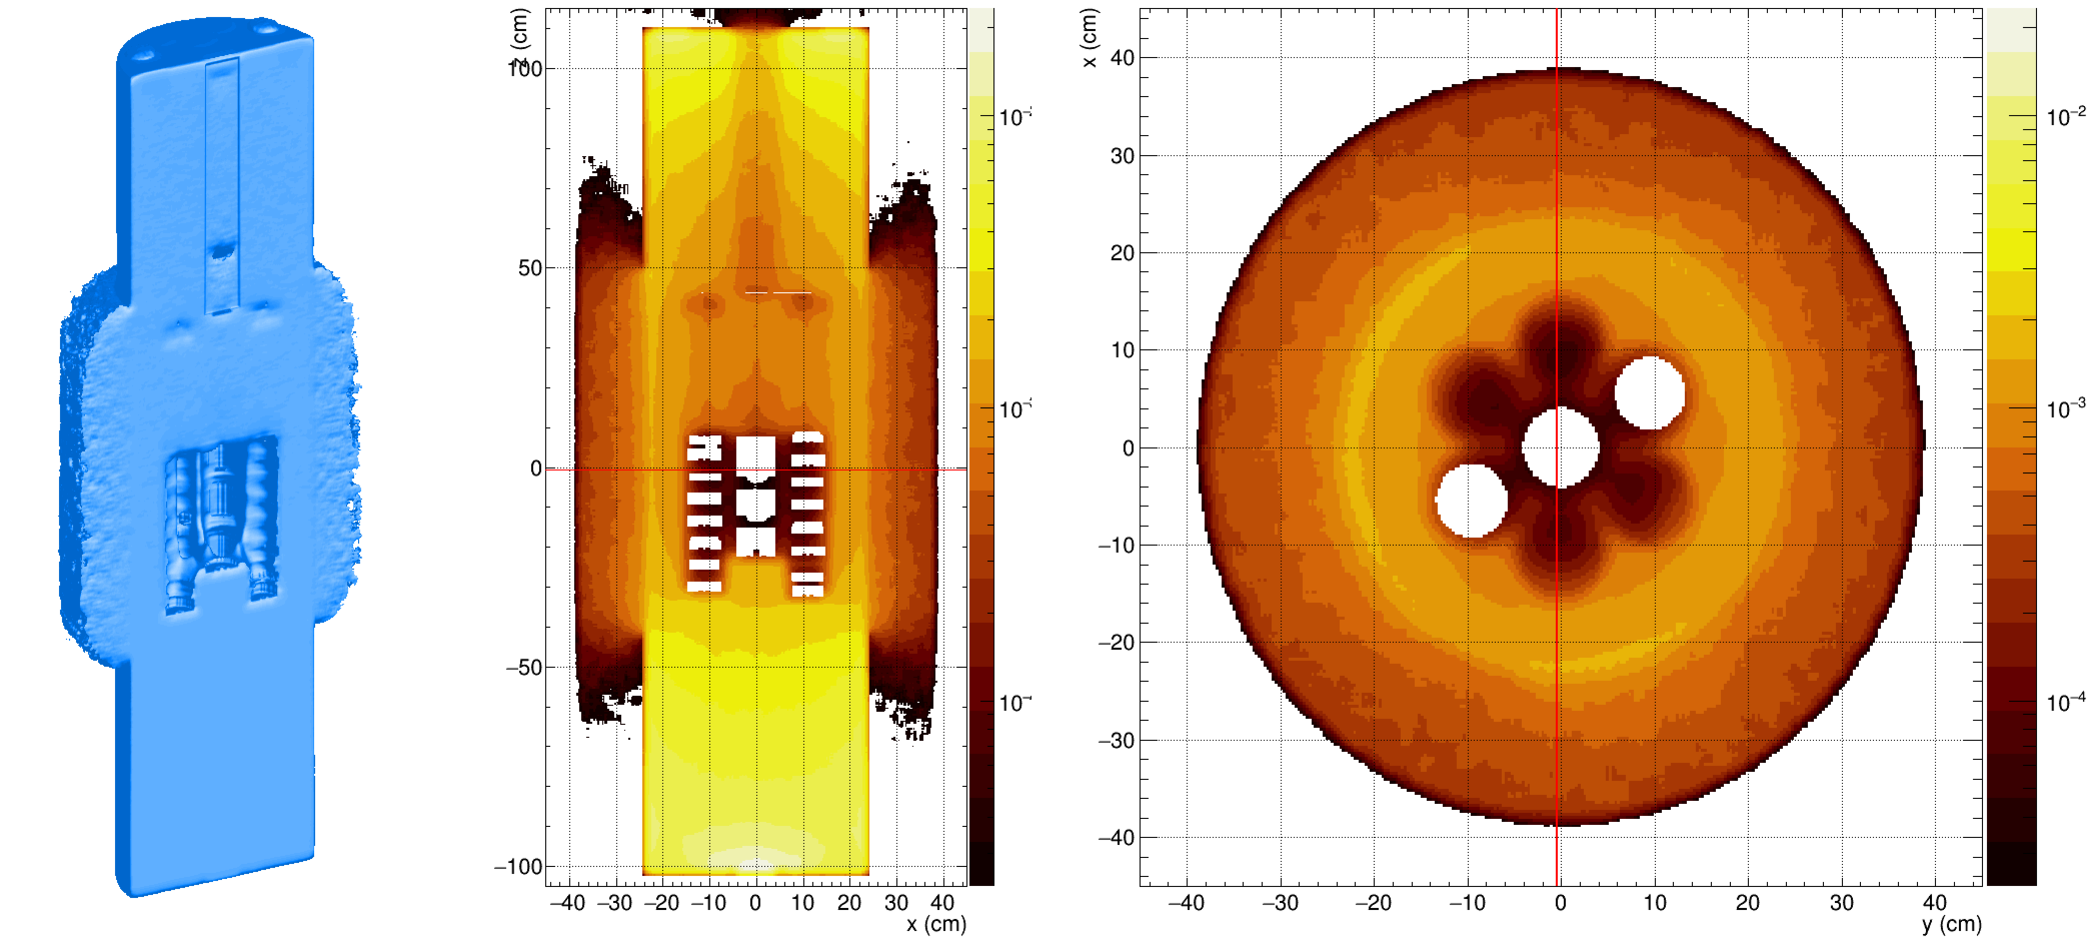
\includegraphics[width=0.9\linewidth]{plots/lar/larmap-tac.png}
  \caption{%
    The three-dimensional LAr photon detection probability map interactive viewer.
    Two-dimensional longitudinal and transversal sections are displayed in the second and
    third pad from the left corresponding to the user pointer position on the 3D
    rendering in the first pad. Red lines mark the cut positions. A smoothing algorithm is
    applied to wash out statistical fluctuations and make the map look more homogeneous to
    the eye.
  }\label{fig:bkg:lar:ph2:larmap:tac}
\end{figure}
\newpar
As remarked in \cref{sec:bkg:lar:ph2:mage}, uncertainties on the optical specifications
implemented in \mage\ can be quite large. Properties like the LAr scintillation yield and
attenuation length, the germanium reflectivity and the TPB quantum efficiency can possibly
have a large impact on the probability map. Other crucial unknowns are the SiPM and PMT
channel efficiencies and the coverage of the fiber shroud, defined as the fraction of
lateral surface area of the curtain occupied by fiber material. Channel efficiencies
extracted from physics data cannot be used, as the simulated efficiencies account for
various other effects in the Monte Carlo and can therefore be quite different. The fiber
coverage on the other hand should be around 0.5, but there could be shrinking phenomena or
single-fiber twists in LAr which could make the real coverage significantly different.
\newpar
To understand the systematic impact of these parameters on the LAr probability map, a
dedicated Monte Carlo study has been performed. A set of representative voxels has been
selected, whose location is documented in \cref{fig:bkg:lar:ph2:larmap:dist}, rightmost
image. For each of these voxels the probability dependence on some Monte Carlo parameters
has been investigated, giving the results displayed in the remaining plots of
\cref{fig:bkg:lar:ph2:larmap:dist}. Voxels have been considered along the central array
axis (green), just outside (blue) and inside (red) the fiber shroud. An additional voxel
has been chosen in the low-probability region between the \GD{89B} and \GD{02D} detectors
(black). Three properties have been taken into consideration for this study: the germanium
reflectivity, the fiber shroud coverage and the LAr absorption length. The reflectivity
has been scaled with a global factor, such that the unit value refers to the value
implemented in \mage. Two qualitatively different trends can be noticed: the reflectivity
and coverage impact is approximately linear in the considered interval, while the
absorption length acts more exponentially on probabilities. The latter is compatible with
the assumption that attenuation in matter generally follows an exponential law, however a
partial saturation effect seems to take place after about 40~cm, when the typical photon
free path length in the \gerda\ setup is reached. Moreover, the impact of a parameter
depends on the voxel location. As instance, the probability in the black voxel between
\GD{89B} and \GD{02D} changes drastically upon different germanium reflectivity
assumptions. On the other hand, orange and Red voxel close to the fibers (where the
calibration sources are) are the most sensitive to modifications of the fiber shroud
coverage.

\begin{figure}
  \centering
  \includegraphics{plots/lar/larmap-dist.pdf}%
  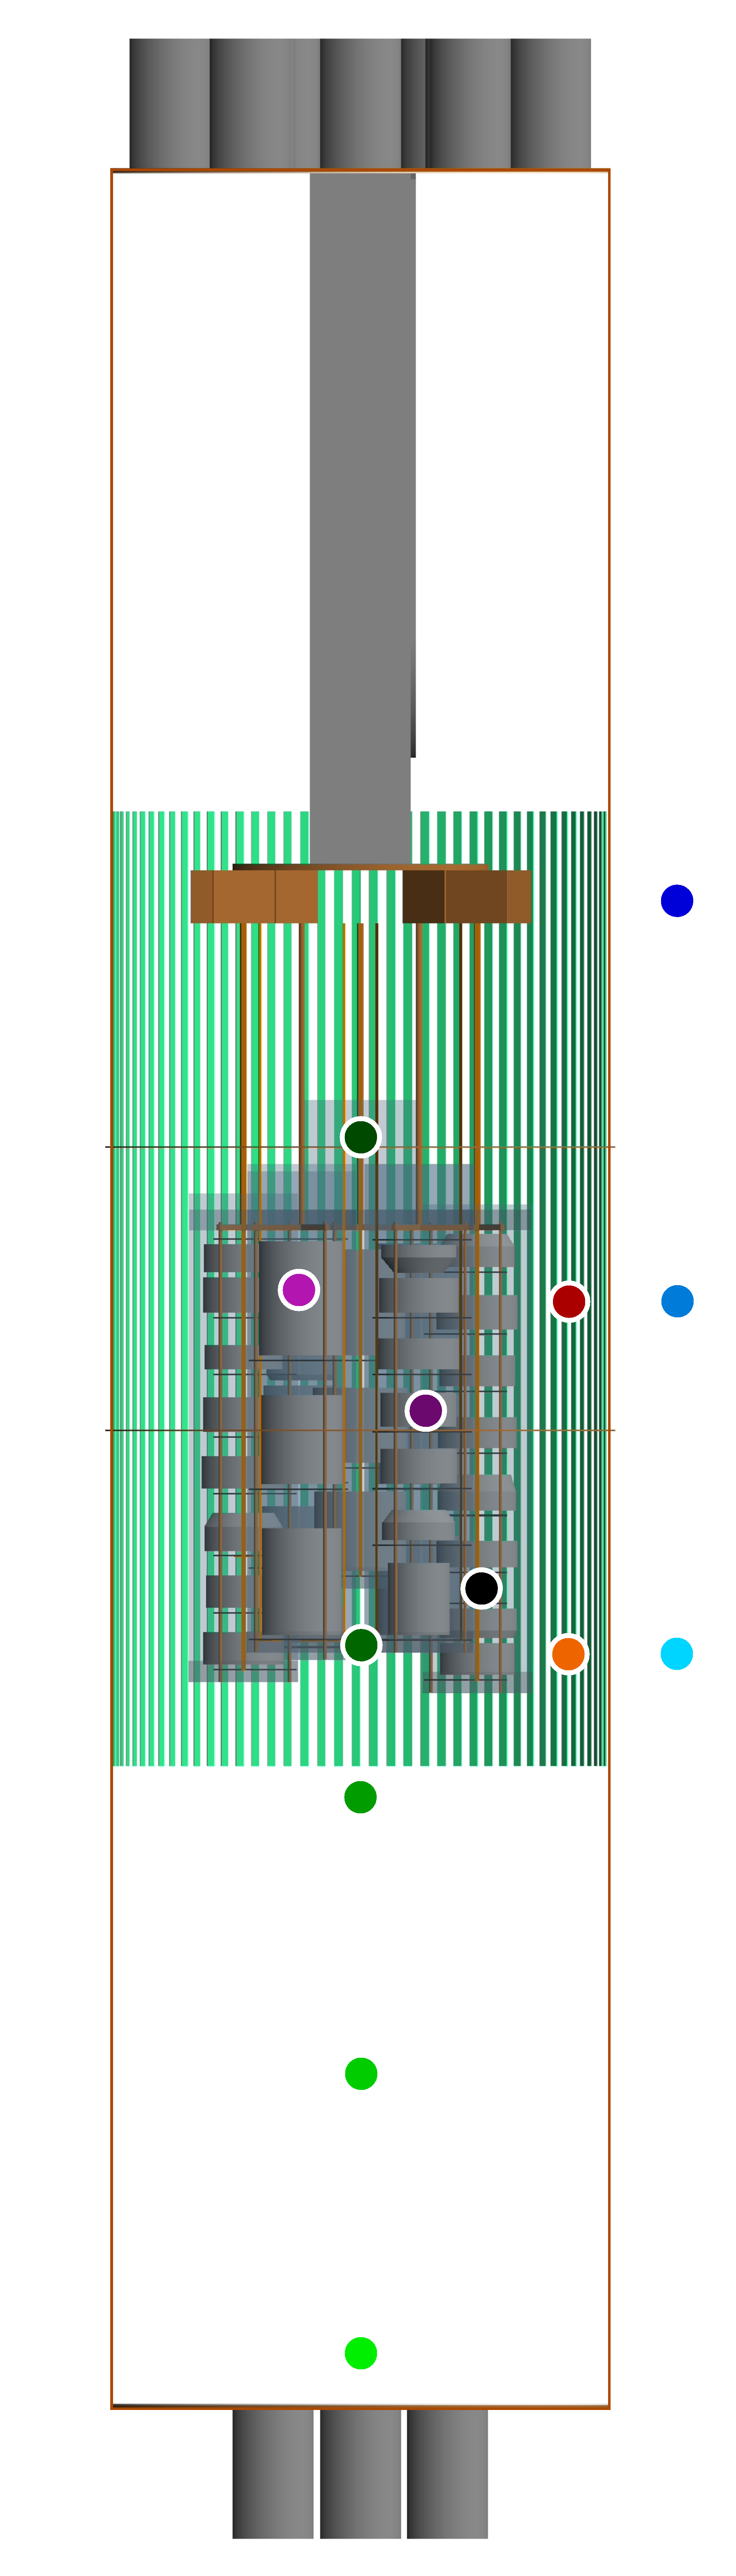
\includegraphics[height=7cm, clip, trim=0 -300 0 0]{plots/lar/lar-points-position.pdf}
  \caption{%
    Study of the impact of Monte Carlo parameters on LAr light detection probabilities in
    various spatial points. Each curve shows the dependence of the probability upon
    germanium reflectivity, fiber shroud coverage and LAr absorption length in the points
    shown in the rightmost scheme of the \gerda\ setup, using the same color code. The
    germanium reflectivity is scaled by a global factor, such that the unit value
    corresponds to the value implemented in \mage.
  }\label{fig:bkg:lar:ph2:larmap:dist}
\end{figure}

\section{Tuning the LAr veto model}%
\label{sec:bkg:lar:ph2:pcalib}

As already mentioned several times, the knowledge about several Monte Carlo optical
specifications is very limited. In particular, PMT and SiPM channel efficiencies are not
known and are essential to build a predictive LAr veto model. Efficiencies extracted from
physics data cannot be used directly, as the Monte Carlo efficiencies are in reality
complex objects that account for other effects. As instance, SiPM efficiencies can include
systematic effects from details of the geometry implementation of the fiber modules in
MaGe. To overcome these issues, a statistical analysis has been developed to tune the
Monte Carlo parameters with physics data. A sample which is independent from the
regular \gerda\ physics data has been identified in the special calibration runs with
low-activity sources and the LAr veto instrumentation turned on.

\begin{table}
  \centering
  \caption{%
    The special calibration runs 68 (July 2016) and 76 (February 2017).
  }\label{tab:bkg:lar:ph2:pcalib-desc}
  \begin{tabular}{lcccc}
    \toprule
    isotope      & source port & position (mm) & lifetime (h) & TP acceptance (\%) \\
    \midrule
    \mr{6}{\Th}  &             & 8168          & 10.2         & no TP              \\
                 & \m{S2}      & 8396          & 3.2          & no TP              \\
                 &             & 8570          & 12.5         & no TP              \\
                 \cmidrule{2-5}
                 &             & 8220          & 6.4          & 92.9(6)            \\
                 & \m{S3}      & 8405          & 4.3          & 93.1(9)            \\
                 &             & 8570          & 3.6          & 90.5(12)           \\
    \midrule
    \mr{6}{\Ra}  &             & 8139          & 8.9          & 89.3(2)            \\
                 & \m{S2}      & 8405          & 4.3          & 90.6(3)            \\
                 &             & 8570          & 6.9          & 88.3(3)            \\
                 \cmidrule{2-5}
                 &             & 8128          & 8.0          & 90.4(2)            \\
                 & \m{S3}      & 8292          & 3.6          & 93.2(3)            \\
                 &             & 8570          & 8.5          & 91.0(2)            \\
    \bottomrule
  \end{tabular}
\end{table}

% vim: tw=90
